\chapter{Simulated data}\label{ch:simulation}

You understood this up to version 3, so this chapter moves quickly. It collects the method in
one place, because the training later depends on it.

\begin{careful}[Synthetic and simulated are two different things here]
The repository has two generators, and it is easy to mix up the words.
\begin{itemize}
\item \textbf{Synthetic data} is the earlier pipeline from October, in \code{scripts/synthetic_data.py}. It makes new pairs by
augmenting real COMSOL fields. It was used for the 1,080-pair experiment, and it is \emph{not} used here.
\item \textbf{Simulated data} is the new generator, \code{scripts/simulate_fields.py}. It computes fields from drawn
wires, and COMSOL never enters it. Everything in this booklet uses simulated data, version 3.
\end{itemize}
\end{careful}

\section{Why simulate at all}

Fifteen pairs from two wire shapes cannot train a network with millions of parameters. So we
need many more examples of the same physics. Your original idea was a spiral with blur and noise.
The final generator goes one step further: it computes the field from a current, so all three
components agree with each other and with Maxwell's equations. This is much easier to defend than
a blurred line drawing.

\section{The recipe, step by step}

\subsection*{Step 1: draw a wire layout}

Each sample starts from a recipe. It picks a family and random settings.

\begin{code*}{simulate_fields.py}
    rng = np.random.default_rng(sample_seed(seed, label))
    family = str(rng.choice(('spiral', 'meander', 'array'), p=(.35, .35, .3)))
    width = float(rng.uniform(*settings['width_um']))
\end{code*}

\begin{itemize}
\item \textbf{Spiral:} a two-arm rectangular spiral, like L1\_C1.
\item \textbf{Meander:} a serpentine with uneven teeth.
\item \textbf{Array:} 2 to 4 mirror copies of one spiral in the image quadrants, like C1+C2+C3+C4.
\end{itemize}

Every path is closed. It leaves the image and returns along a rail 35\um\ outside, because real
current must flow in a loop. The code redraws a layout if any wires come too close. Each sample also
gets a random width of 1.6--3.2\um, a source offset of 0--0.2\um, and a noise level of 1, 1.5, 2 or
2.5\%. The current is fixed at 600\textmu A, the same as COMSOL.

\subsection*{Step 2: turn the wire into a current map}

\code{rasterize} paints the wire onto a pixel grid as two arrays, $K_x$ and $K_y$, the sheet current
density in A/m. It uses partial pixel coverage so edges are not jagged. At a corner two wires overlap,
so the current there is shared equally.

\begin{code*}{simulate_fields.py}
    # Both wires cover a corner square; share the current between them there.
    corner = (kx != 0) & (ky != 0)
    kx[corner] /= 2
    ky[corner] /= 2
\end{code*}

The canvas has 700 pixels of padding on each side, so the Fourier transform does not wrap
fields around the image edges.

\subsection*{Step 3: compute the field from the current}

This is the thin-sheet Biot--Savart law in Fourier space. With $k=2\pi|f|$ and $d$ the source offset:
\begin{align}
E(k,z) &= \frac{\mu_0}{2}\, e^{-k(z+d)},\\
B_x(k) &= E\, K_x(k),\\
B_y(k) &= E\, K_y(k),\\
B_z(k) &= E\, \frac{i\,(k_y K_x(k) - k_x K_y(k))}{k}.
\end{align}

\begin{code*}{simulate_fields.py}
    fx, fy = np.fft.rfft2(kx), np.fft.rfft2(ky)
    # Drawn corners leak a little current; remove the divergent part so the
    # in-plane fields describe the same conserved current as Bz.
    longitudinal = (wx * fx + wy * fy) / safe ** 2
    fx, fy = fx - wx * longitudinal, fy - wy * longitudinal
    fz = 1j * (wy * fx - wx * fy) / safe
    fx[0, 0] = fy[0, 0] = fz[0, 0] = 0
\end{code*}

Notice that one current map gives all three components at both heights. Nothing is drawn separately.

\begin{keyidea}[The target and the input come from the same physics]
The same formula runs twice, at $z=0.5$ and $z=3$. So the training pair is consistent with the
operator $h$ by construction.
\end{keyidea}

\begin{careful}[The labels look swapped, and that is deliberate]
In real physics, $B_x$ is driven by $K_y$. Here $B_x$ uses $K_x$. That is because the COMSOL
export frame is rotated 90 degrees from the image axes. Bx and By only satisfy Maxwell's
equations with Bz when the frame is rotated: the residual is 10.9\% rotated and about 100\% as
labelled. The generator copies the COMSOL frame.
\end{careful}

\subsection*{Step 4: add COMSOL-like noise, to the input only}

COMSOL fields carry a fine speckle tied to the mesh. Measured from mirrored coils, it has a range of
1.4--1.9\% for $B_x$ and $B_y$, 2--3.4\% for $B_z$, and a correlation length of about 0.38\um. So the
generator adds noise that is correlated over that same length.

\begin{code*}{simulate_fields.py}
def correlated_noise(white, corr_um, dx):
    """Unit-variance noise with exponential spatial correlation length corr_um."""
    ny, nx = white.shape
    fx = np.fft.rfftfreq(nx, dx)[None, :]
    fy = np.fft.fftfreq(ny, dx)[:, None]
    f2 = fx ** 2 + fy ** 2
    amplitude = (1 + (2 * np.pi * corr_um) ** 2 * f2) ** -0.75
    field = np.fft.irfft2(np.fft.rfft2(white) * amplitude, s=(ny, nx))
    return (field - field.mean()) / field.std()
\end{code*}

Noise goes on the input only. The target stays clean. So the network is asked to remove speckle
as well as blur.

\subsection*{Step 5: normalise}

All fields are divided by one number: 145.487\muT, the largest peak among the training targets.
COMSOL is divided by the same number, and it never helps choose that number.

\begin{figure}[H]
\centering
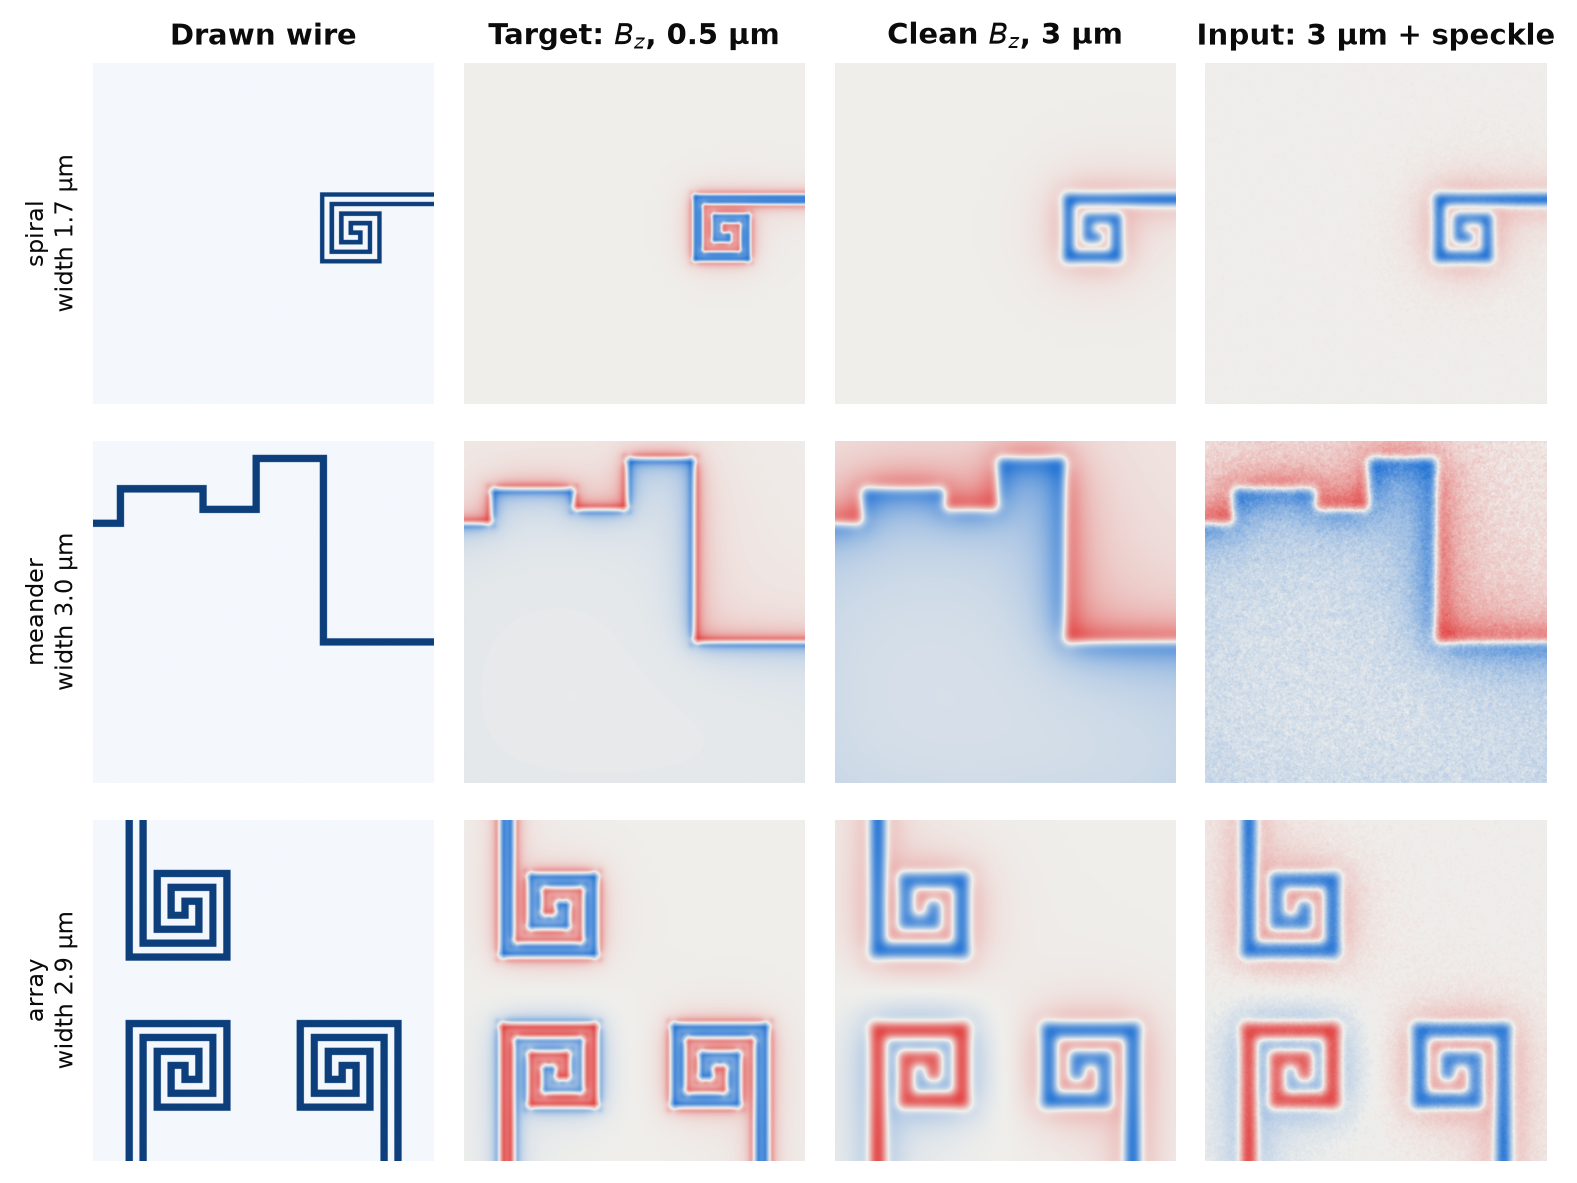
\includegraphics[width=\textwidth]{simulated}
\caption{Three training layouts from v3, one from each family. Only $B_z$ is shown. The right two
columns share a colour scale, so the speckle is visible in the input.}
\label{fig:simulated}
\end{figure}

\section{How v1 became v3}

\begin{center}
\begin{tabularx}{\textwidth}{lX}
\toprule
Version & What it had \\
\midrule
v1 & One wire per sample, free-space decay, white noise \\
v2 & Added array layouts and correlated speckle, plus an empirical decay $k_0=0.095$ rad/\textmu m
that mimics COMSOL's faster fall-off \\
v3 & Same layouts as v2, with $k_0$ removed. Pure free-space physics. This is the dataset used \\
\bottomrule
\end{tabularx}
\end{center}

\begin{keyidea}[Why $k_0$ was removed]
COMSOL fields decay faster with height than free-space physics allows, and the cause is unknown.
A term like $k_0$ fits this, but it breaks the law that a static field above its sources must
obey. You rejected it, and the operator stayed $e^{-kz}$. The mismatch is small at 3\um\ and large
by 10\um, which is one more reason to work at 3\um.
\end{keyidea}

\section{What was generated}

\begin{center}
\begin{tabular}{lr}
\toprule
Item & Value \\
\midrule
Training layouts & 200 \\
Validation layouts & 50 \\
Component pairs & 750 \\
Families & 80 spirals, 97 meanders, 73 arrays \\
Size on disk & 536 KB of recipes \\
\bottomrule
\end{tabular}
\end{center}

The dataset stores recipes, not images, and regenerates arrays when needed. The split is by
layout, so a validation wire is never seen in training.

\section{How realistic is it?}

To check the physics, the real L1\_C1 coil was rebuilt from its traced centreline and compared with
COMSOL.

\begin{center}
\begin{tabular}{lccc}
\toprule
Height & $B_x$ error & $B_y$ error & $B_z$ error \\
\midrule
0.5\um & 16.8\% & 18.8\% & 23.0\% \\
3\um & 12.7\% & 13.8\% & 25.8\% \\
10\um & 63.7\% & 64.1\% & 139.7\% \\
\bottomrule
\end{tabular}
\end{center}

So the simulator is close at our two heights and fails at 10\um.

\begin{careful}[Limits of the simulator]
\begin{itemize}
\item The wire width and offset for that check were fitted on the same coil, so it is a regression
check, not independent proof.
\item COMSOL's speckle sets a floor. Even a perfect clean model cannot score below about 15--19\%
against COMSOL at 0.5\um, because that much of the COMSOL target is mesh speckle.
\item Every COMSOL peak lies above the simulated range, so the spikes are not modelled.
\item Fifteen automated tests pass, covering closed-form loop and strip fields, Maxwell
consistency, and repeatability.
\end{itemize}
\end{careful}
